\section{Tracking with the Inner Detector} \label{sec:atlas:tracking}

With its closest component, the insertable b-layer (IBL)
\cite{Potamianos:2209070}, only 3.3 cm from the beampipe The Inner Detector
(ID), shown in figure \ref{fig:inner_detector_diagram}
\cite{ATLAS-TDR-4,ATLAS-TDR-5} faces the incredible challenge of providing
precision momentum resolution and identification of both primary and secondary
vertex measurements of charged tracks all while recieving the highest fluence of any detector.

\begin{figure}[!htbp]
  \begin{center}
    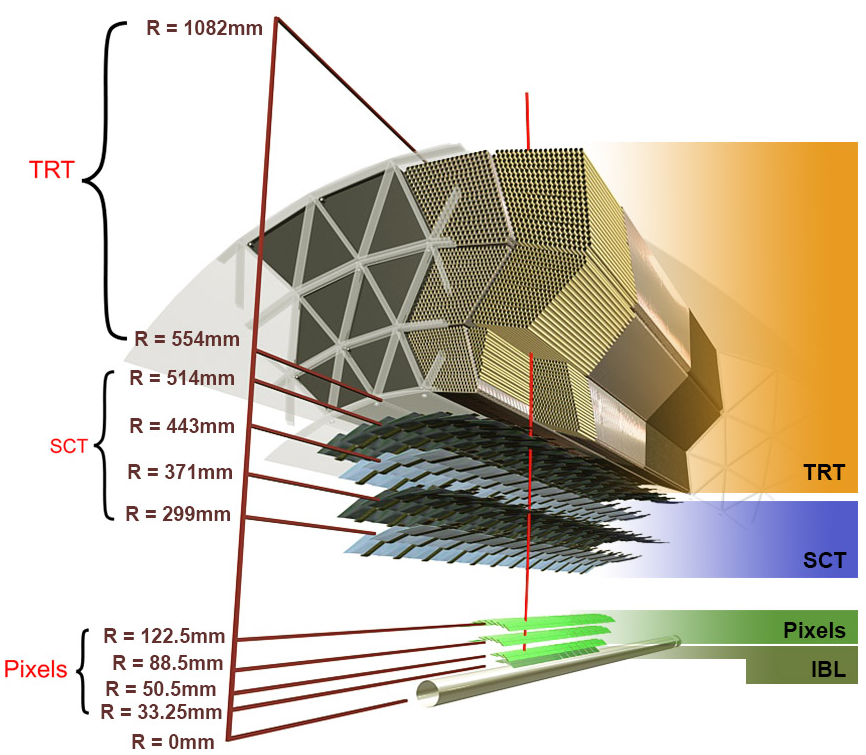
\includegraphics[width=0.8\linewidth]{figures/atlas/inner_detector_diagram}
    \caption{ \cite{Potamianos:2209070} Diagram of inner detector}
    \label{fig:inner_detector_diagram}
  \end{center}
\end{figure}

It is designed to be very compact to fit inside the 2T solenoid and to give
excellent momentum resolution above the nominal \pT threshold of $0.5$GeV and
within the pseudorapidity range of $|\eta| < 2.5$ as shown in figure \ref{fig:inner_detector_schematic}

\begin{figure}[!htbp]
  \begin{center}
    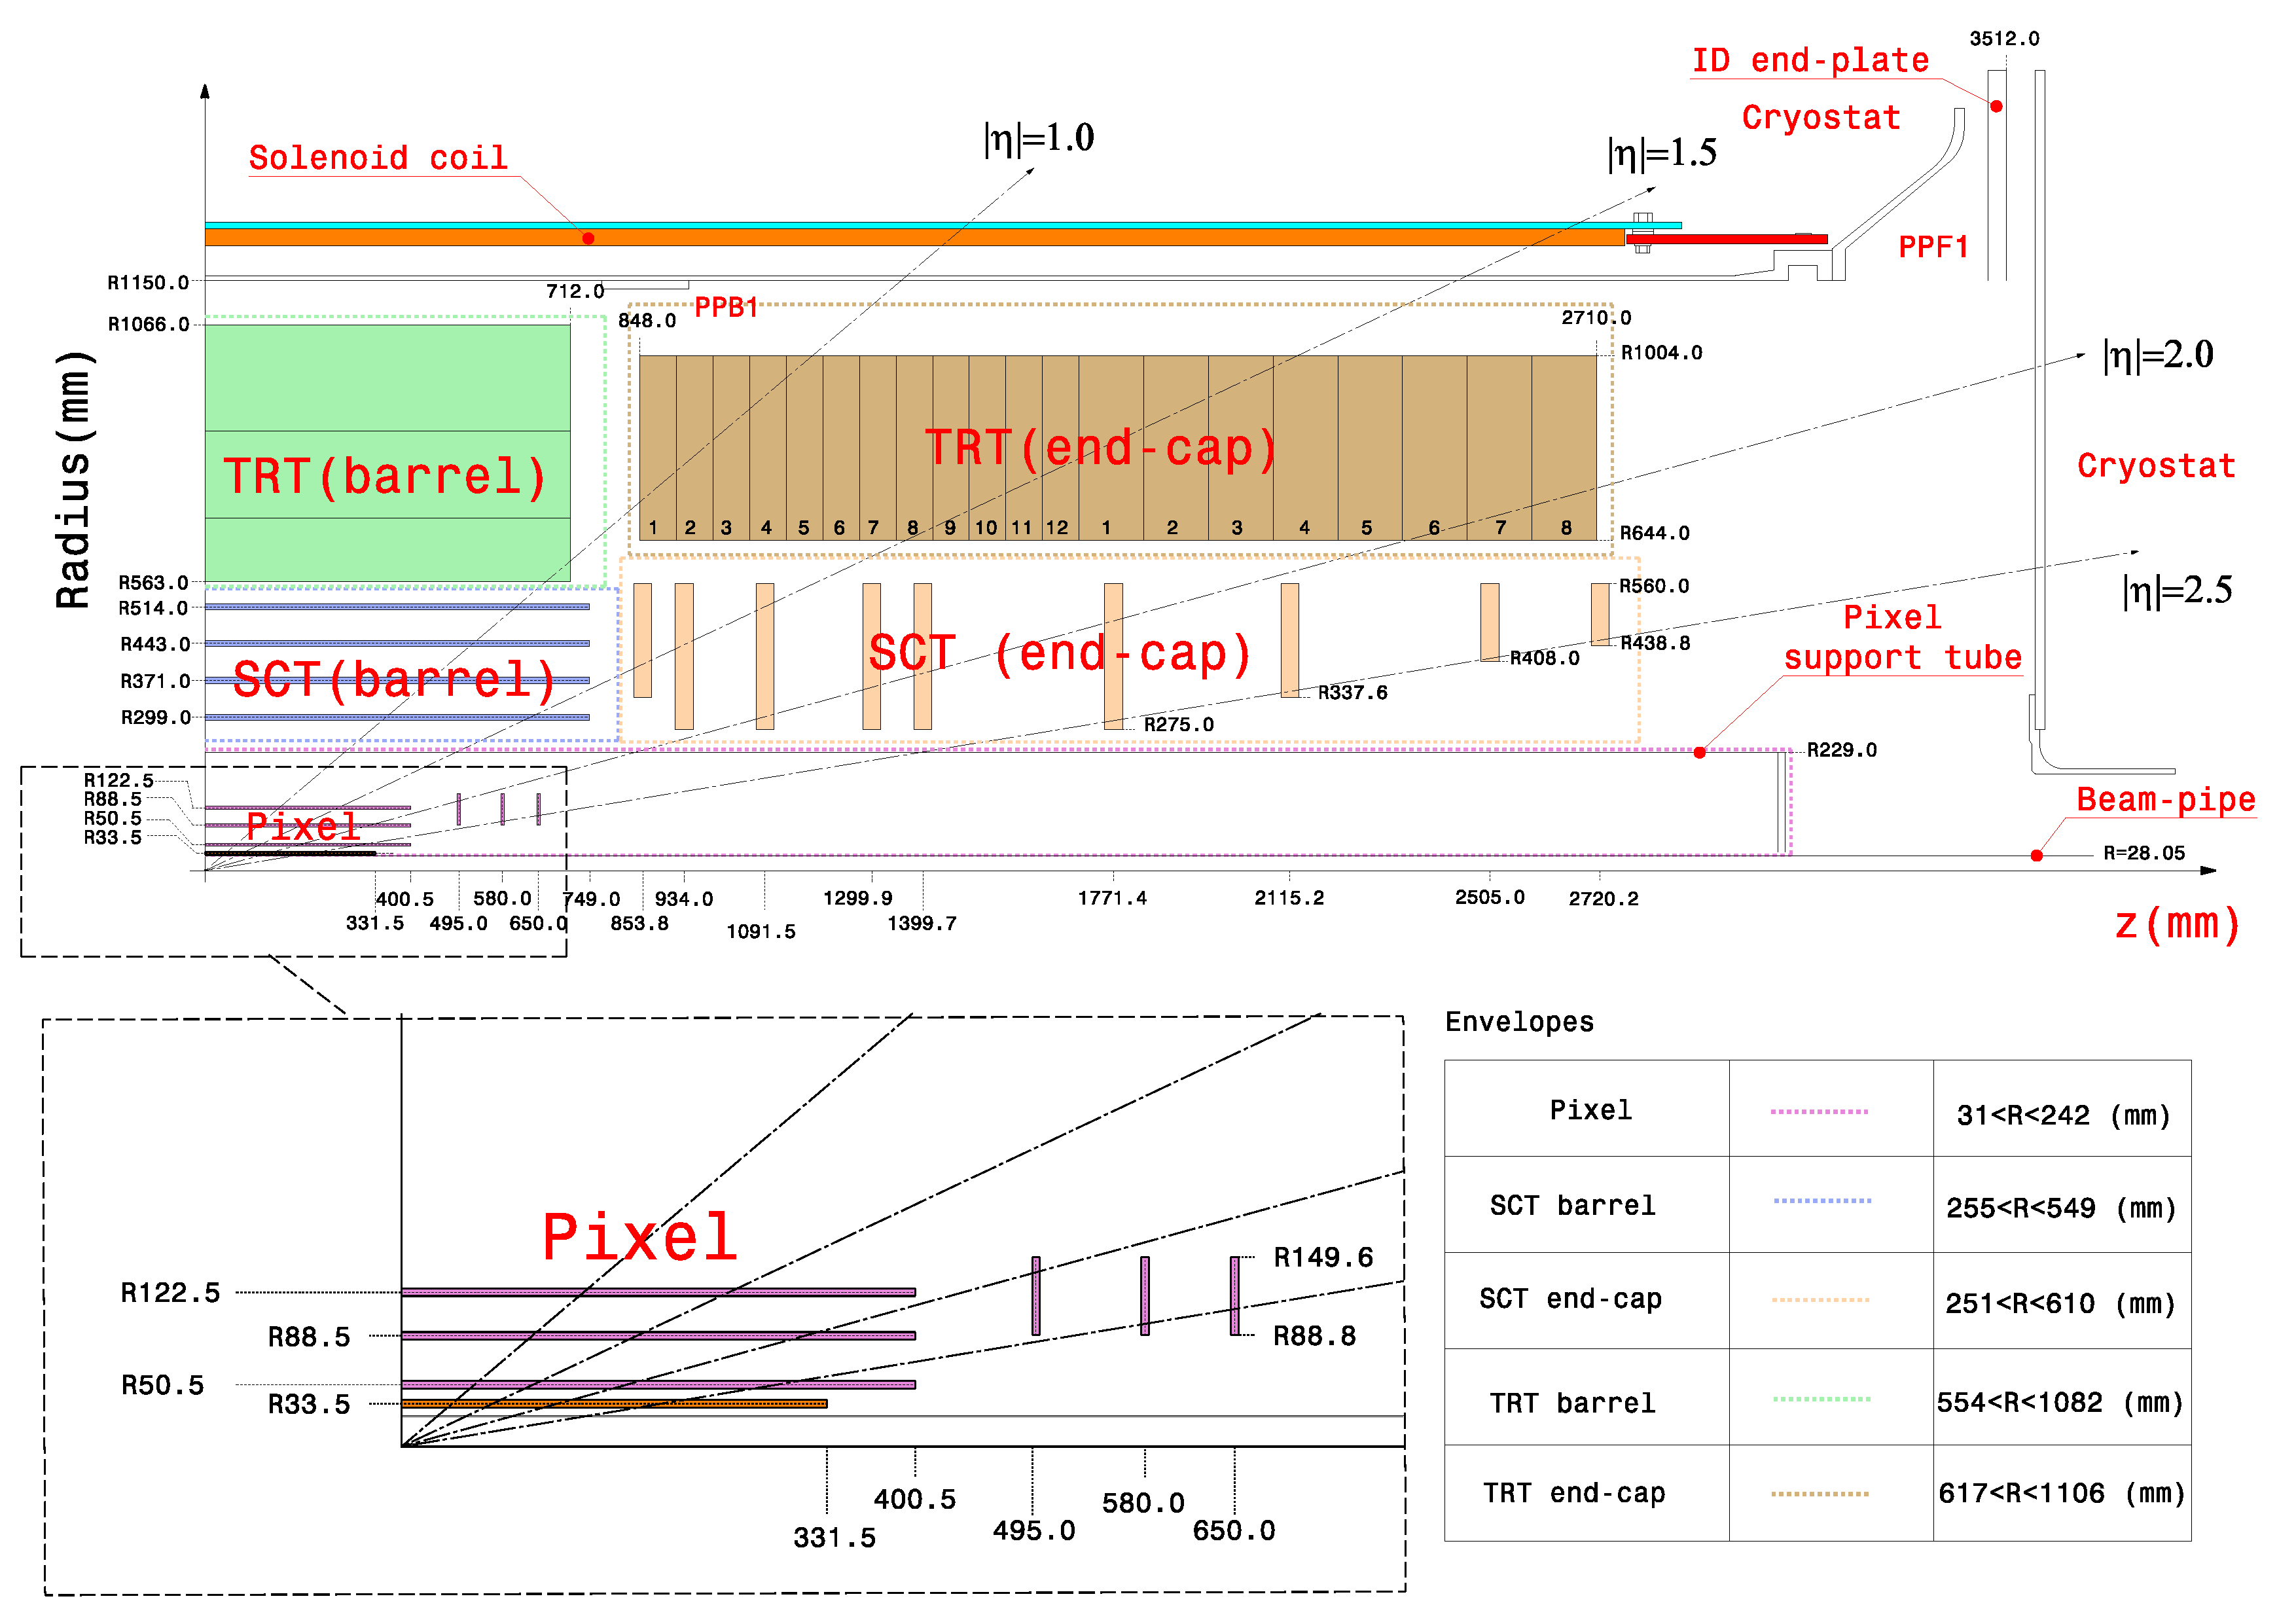
\includegraphics[width=0.8\linewidth]{figures/atlas/inner_detector_schematic}
    \caption{ \cite{PIX-2018-001} Schematic of the Inner Detector including eta lines}
    \label{fig:inner_detector_schematic}
  \end{center}
\end{figure}

